\chapter{Symbolic Derivation}

We give a detailled description of how automatic differentiation is handled in {\tt MMVII}.
This description is for programmer who will have to maintain this part or possibly also for curious readers .
However we recommand to read before the short introduction given in~\ref{Compute:Deriv:SysNL} (or better all chapter~\ref{Chap:NLO}) to
have a better understanding of where we go.

For devlopper that will only be users of these  automatic differentiation facilities in {\tt MMVVII} , probably
~\ref{Compute:Deriv:SysNL} or~\ref{Chap:NLO} is sufficient.


%-----------------------------------------------------
%-----------------------------------------------------
%-----------------------------------------------------

\section{introduction}


%-----------------------------------------------------
\subsection{Motivations}

The computation of derivatives of a given function is a central point in metrology
where it is used in Gauss-Newton-like iteration.  There is basically $4$ methods
for computing derivatives :

\begin{itemize}
    \item  computing "by hand", i.e a human apply the rules of derivation as
           learned at school;  for small formula, this method is perfectly manageable 
           and also probably the fastest when the code is optimized;
           but with "complicated" function, as colinearity equation with many distorsion parameters,
           it is error prone, difficult to maintain, and potentially not so fast as there
           are simplifications that human may miss;

    \item  numericall derivative: for example with a $2$ variables function, we use equation as~\ref{NumDer}
           where $\epsilon_x$ is a "small" value relative to variable $x$;
           this method has the advantage of simplicity, if you know the function you know its derivatives;
           it has $2$ drawbacks :  first issue, it's not always easy to define a good small value, a too small value
           creates numericall problem, not enough small is unacurate, all the more with heterogeneous variable the "small"
            value must be re-defined for each variable;  second issue, it is relatively slow, with $N$  variables
           we must have $2N$ evaluations of $F$;

     \item jet method as used in CERES, see~\cite{CERES} for detailled description, it's not error
           prone as "hand crafted", there is no problem of accuracy, they are faster than 
           numerical derivatives; however they are relatively slow compared to formal methods;

   \item formal method, that "more or less" do the same thing than "human computation" (generate the
	   analyticall formula) but do
           it automatically; they are separated between automatic differenciation that analyse the code of a programm
           and symbolic differenciation that construct a tree representation, but to our mind this separation
           is a bit artificial : they are conceptually close and 
           their performance are similar;  {\tt MMVII} uses symbolic differenciation;
           the use is a bit more complicated than jet but can be significatively faster  on complicated
           formulas.
\end{itemize}

\begin{equation}
    \frac{\partial F(x_0,y_0)}{\partial x} \approx \frac{F(x_0 + \epsilon_x,y_0) - F(x_0-\epsilon_x,y_0)}{2* \epsilon_x}
     \label{NumDer}
\end{equation}

%-----------------------------------------------------
\subsection{Code localization}

The code on automatic differenciation has been organized in such a way that 
the code can be reused outside the {\tt MMVII} library. It's a header only code
that is located in {\tt MMVII/include/SymbDer/}.


The code that use it more specifically for task adressed in  {\tt MMVII},
as photogrammetry or compensation in general, are to be found in the
folder  {\tt MMVII/src/SymbDerGen}.


%-----------------------------------------------------
\subsection{Tree/DAG representation}

\begin{figure}
\centering
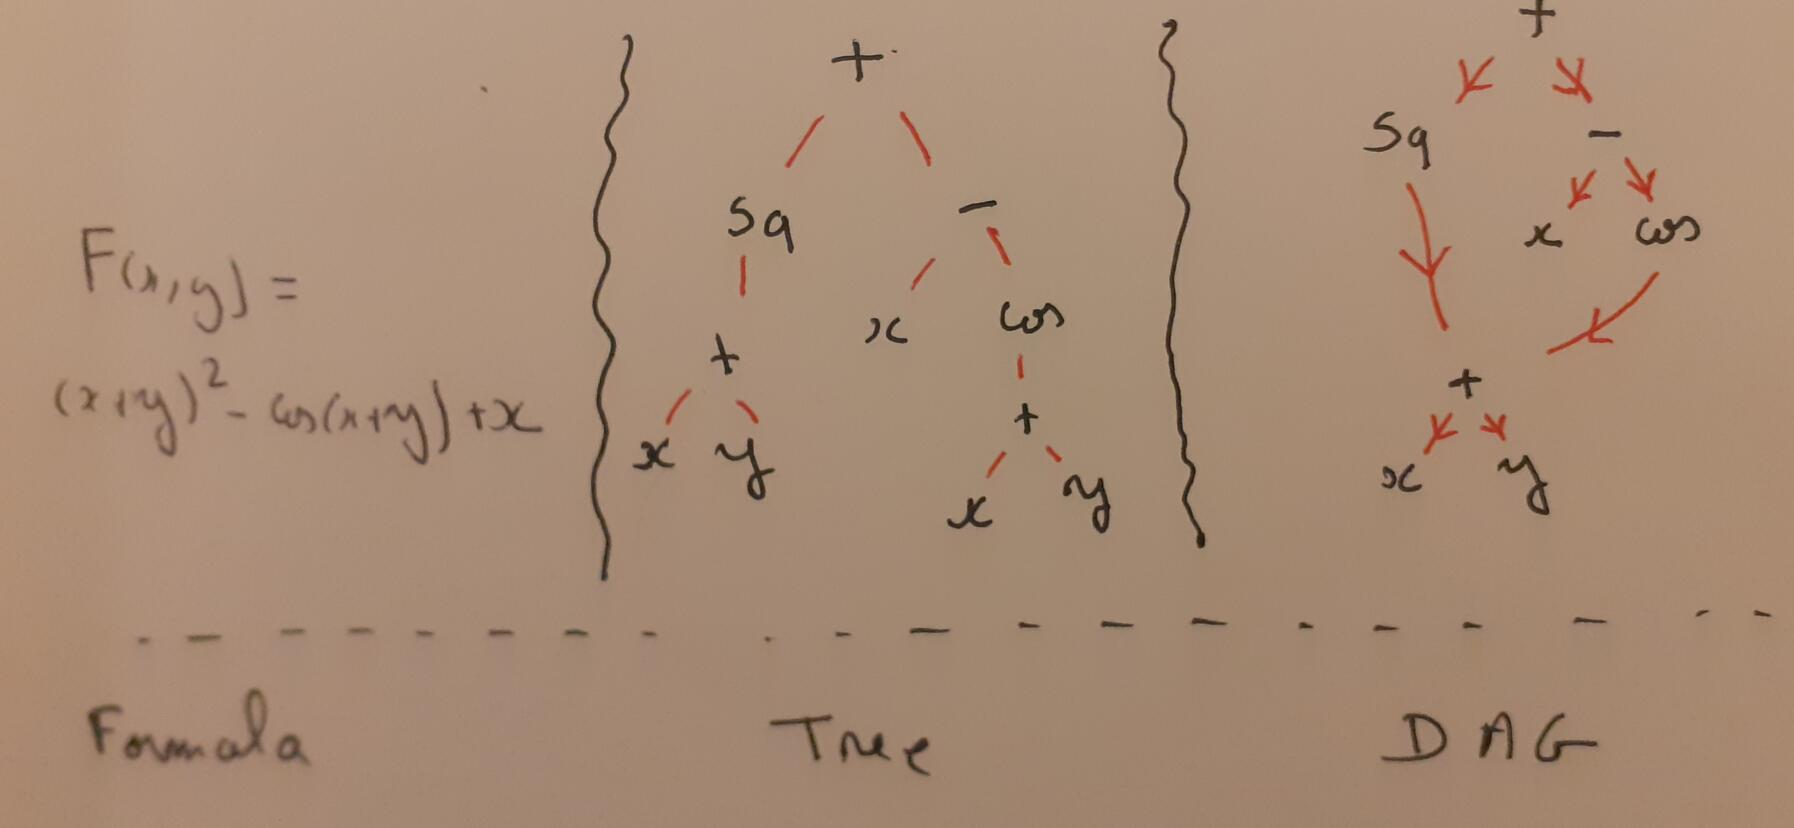
\includegraphics[width=12cm]{Programmer/ImagesProg/Tree.jpg}
\caption{Representation of formulas}
\label{fig:TreeFormula}
\end{figure}

A classic aproach in computer science is to represent mathematicall formulas 
as trees (or more precizely as we will see as "DAG"=  directly acyclic graph).
These trees can be described recursively :

\begin{itemize}
   \item  constant ($0,1,\pi \dots$)  and fonctions corresponding to variables ($x_1,x_2,\dots ,x_{144} \dots$)
          are  atomic formulas, their tree has one node labeled by the contant or the variable;

   \item if $Op$ is a unary operator, like $\cos, \sin, \exp $ for example,  and $F$ is a formula then $Op(F)$ is a 
         formula, its tree is a node labeled by $Op$ and has one son corresponding to the tree of $F$;

   \item if $Op$ is a binary operator, like $+,*,pow $ for example,  and $F_1$  and $F_2$ are 
	   formulas then $Op(F_1,F_2)$ (or $F_1 Op F_2$ in infix notation) is a 
         formula,  its trees is a node labeled by $Op$ and has two son corresponding to the trees of $F_1$ and $F_2$.
\end{itemize}


Figure~\ref{fig:TreeFormula} represent the tree for the formula $F(x,y) = (x+y)^2 +x - \cos(x+y)$. 
In the formula, we see that the sub-formula $x+y$ appears twice , then to optimize the computation,
a directed acyclic graph (DAG) is prefered to tree;  a DAG  is still a hierarchy, but the difference
if that a node can have several parents, which avoid duplication as the same formula can be shared.
The right part of figure~\ref{fig:TreeFormula} correspond to DAG for formula $F$.
When we will generate the code, we will set a variable on the shared node, for example $V_{577} = x+y$ , and then reuse
this variable when we need it instead of redoing computation.


The difference in efficiency between a tree and a DAG can be very significant 
in complicated multiple formula  (maybe up to $10$ in colinearity). By multiple formula we mean formula that return several values;
in differenciation we will compute $F$ but also all its derivatives and it often happen that
the same sub-formula appears in several partial derivatives.  In our example we
have $\frac{\partial F}{\partial x} = 2*(x+y) -1 + \sin(x+y)$ and $\frac{\partial F}{\partial y} = 2*(x+y) + \sin(x+y)$ ,
and figure~\ref{fig:DagMultiformula} represents the DAG for the multiple formula
$\{F,\frac{\partial F}{\partial x},\frac{\partial F}{\partial y}\}$.



\begin{figure}
\centering
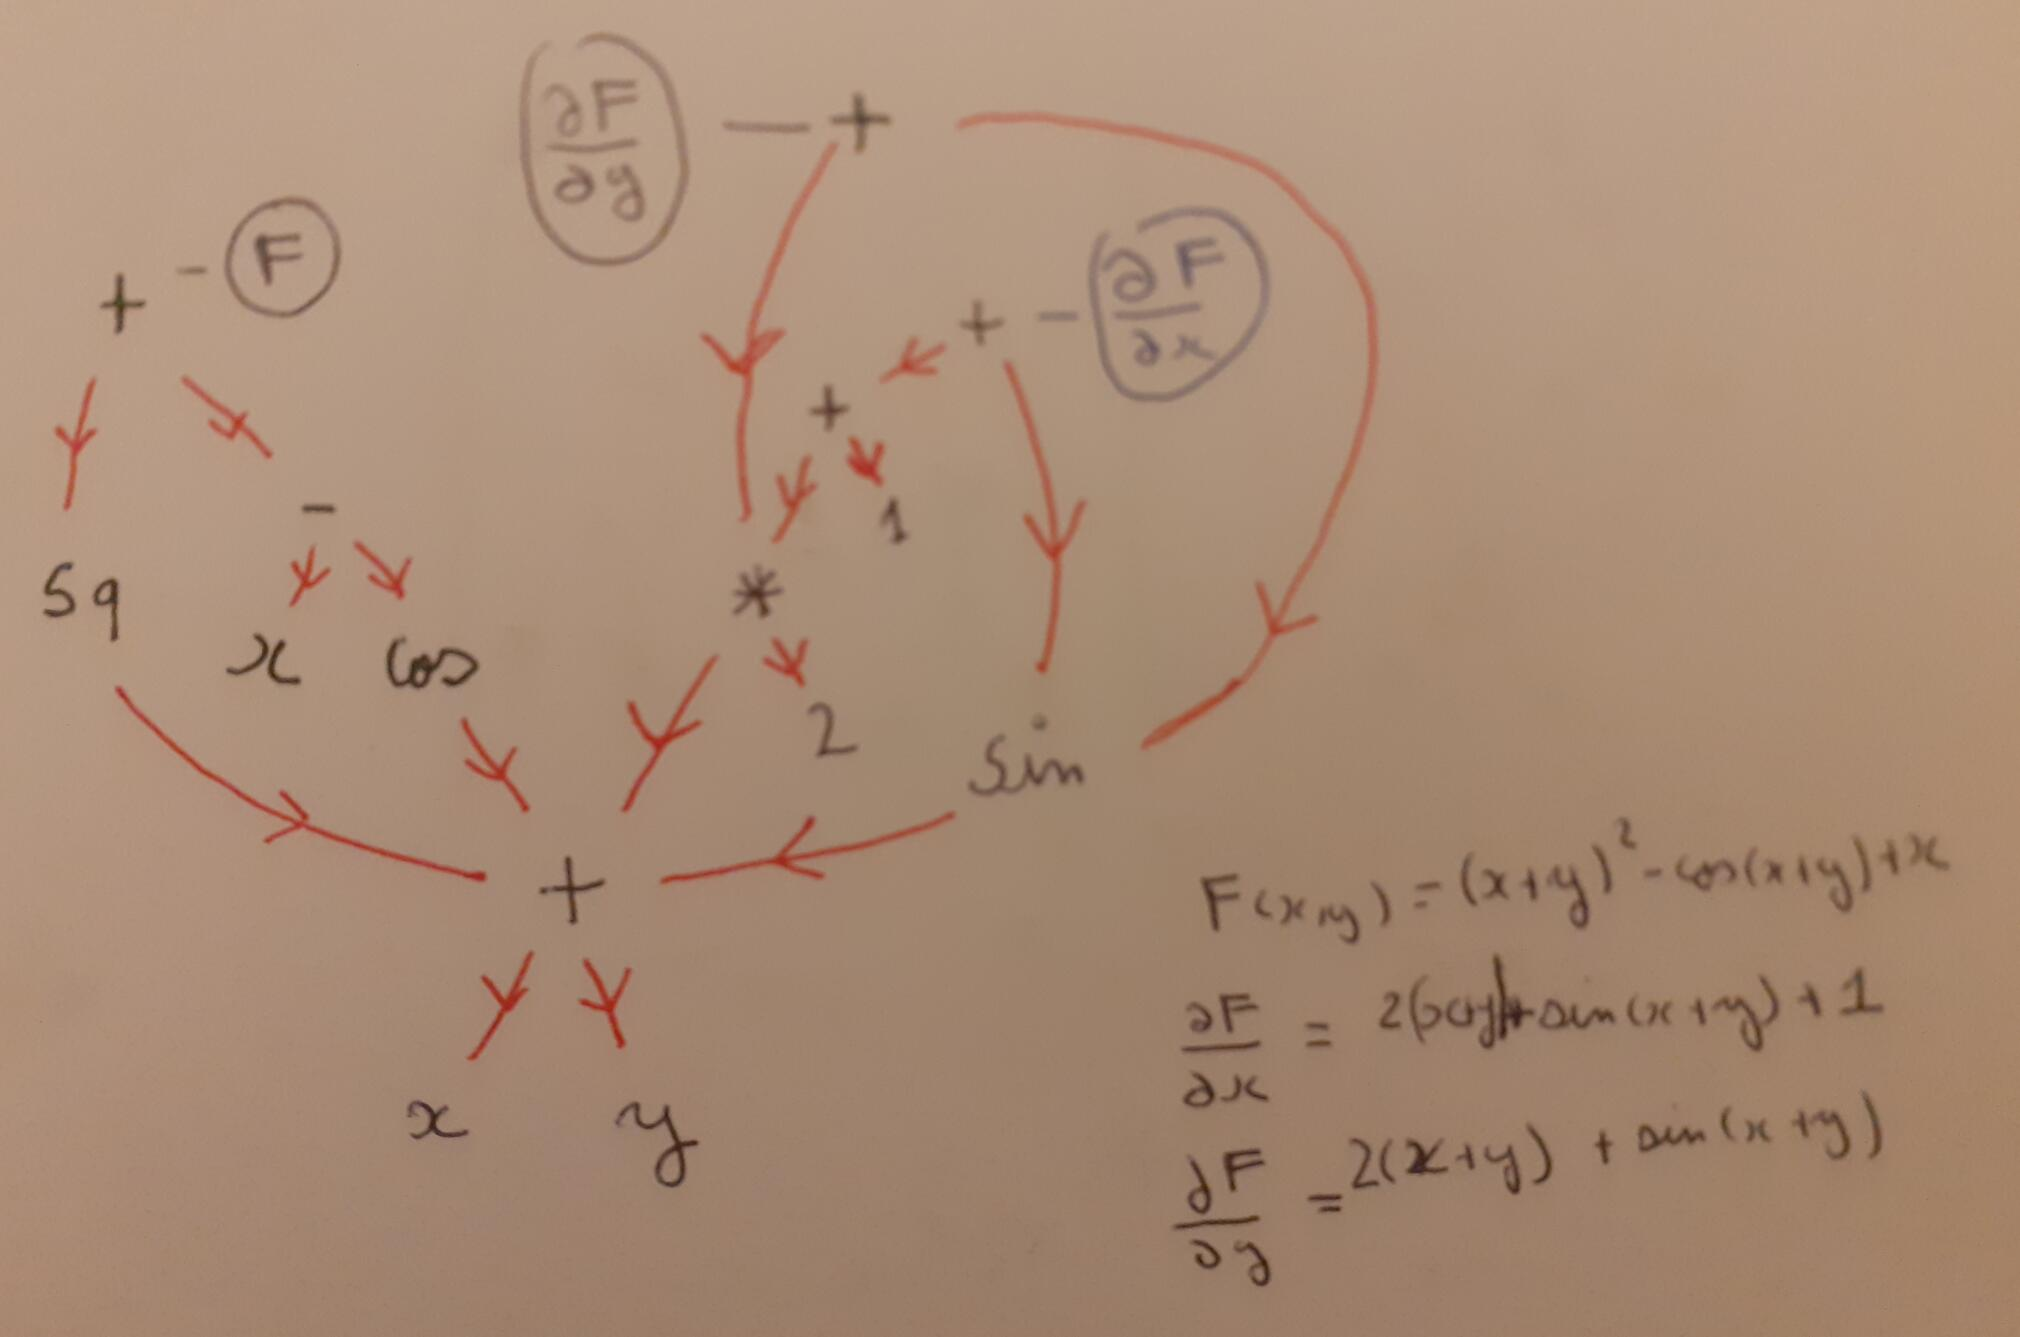
\includegraphics[width=12cm]{Programmer/ImagesProg/DAG.jpg}
\caption{DAG for a multiple formula  $[F,\frac{\partial F}{\partial x}, \frac{\partial F}{\partial y}]$ with $F(x,y) = (x+y)^2 +x - \cos(x+y)$}
\label{fig:DagMultiformula}
\end{figure}


%-----------------------------------------------------
%-----------------------------------------------------
%-----------------------------------------------------

\section{General organization}

%-----------------------------------------------------

The code is located in  {\tt MMVII/include/SymbDer/}.

\subsection{formulas}

The key-file is {\tt SymbolicDerivatives.h}  where is defined   the key-classes   {\tt cFormula and cImplemF},
cFormula being simply pointer on cImplemF,  ({\tt cImplemF} is the real class containing the data, while
{\tt cFormula} are the classes manipulated externally as we want a remanent objet  semantic).
For now we will speak of formula to name undifferrently these two linked classes.


A formula is the {\tt C++} equivalent of the tree/DAG, basically formula work this way :

\begin{itemize}
       \item  a formula contains a set of sub-formula (currently between $0$ en $2$);

       \item  for each kind of formula there is a derived class (i.e one derived class for each operator)

       \item  mathematical operator ($+,*\dots ,\cos,\tan,\dots$) have been overloaded on formula, 
               for example consider a binary operator  $\otimes$ , each time we meet $F_1\otimes F_2$ 
		the rule is to create a new formula of the adequate derived class $c\otimes$ with  
		$\{F_1,F_2\}$ as set of sub-formula,
		there is two (very frequent) exception to this creation of new formula:

               \begin{itemize}
                    \item if the formulla has already be encontered inside a computation, this formula is returned
                          and nothing is created (that why it's a DAG);
		  \item if some simplication rule specific to the operator exist (like $F*1=F$) they are applied;
               \end{itemize}
	       
        \item  a formula contains several virtual methods indicating how to 
               \begin{itemize}
		       \item  compute its value (used in interpreted mode, not usefull for code generation)
		       \item  computes its derivative by return a new formula;
		       \item  computes the generated code;
               \end{itemize}

		the above listing extract these $3$ methods for the {\tt cMulF} correspondingto the multiplication
		of functions;
\end{itemize}


\begin{lstlisting}[language=c++]
// method for computing values
void ComputeBuf(int aK0,int aK1) override
{
    for (int aK=aK0 ; aK<aK1 ; aK++)
        mDataBuf[aK] =  mDataF1[aK] * mDataF2[aK];
}
// === Extract of code in class cMulF (multiplication of formulas )

// method for computing the derivative
cFormula<TypeElem> Derivate(int aK) const override
{
   return  mF2*mF1->Derivate(aK) + mF1*mF2->Derivate(aK);
}

// method for generating the code
std::string GenCodeDef() const override 
{
    return "(" + mF1->GenCodeRef() + " " + this->NameOperator() +  " " + mF2->GenCodeRef() + ")";
}

\end{lstlisting}

%-----------------------------------------------------

\subsection{Coordinator}

Generating the DAG, requires some coordination between the formulas created.
As we want to create a DAG with  minimal number of nodes, we must keep track
of all already existing formulas created for a specific task.
This is where the class {\tt cCoordinatorF} is usefull,  it creates a dictionnary ({\tt std::map})
that stores the association "name/Formula created".  So the coordinator "knows" all the 
formula that belongs to it while each formula "knows" its coordinator. Also the coordinator
associates to each new formula a unique number.

Let illustrate on an example how it works :

\begin{itemize}
	\item  suppose the code contains  $F_1\otimes F_2$  (or  $\otimes(F_1,F_2)$ );
	\item  when this code is executed, $F_1$ and $F_2$ have been created and are given as
		parameter to $\otimes $ (overloaded on formulas), the coordinator has
		attributed a unique number $N_1$ and $N_2$ to these formulas;
	\item  in the function {\tt cGenOperatorBinaire::Generate}, an identifiant is computed $Id="\otimes \; N_1 \; N_2" $,
	\item  if there is a value associated to $Id$, this value is returned, else a new formula is created 
	       the association "Name/formula" is memorized in its coordinator dictionnary, and this new value is returned;
\end{itemize}

The coordinator  is the access point for generating the code. The user has first to select the curent formulas :
it can be the formulas themselves or the formulas plus all their derivatives.
Note that we have the possibility to give several formulas (in a {\tt std::vector}) as curent formulas,
this is because, due to DAG reduction,  the  DAG of $N$ formulas will have less nodes
than the $N$ independant DAG and consequently the code will be more efficient.

Also why would a user generate code without derivatice while
obiously these classes are interesting because we want to compute derivatives? 
In fact  it can be interesting for a given formula to use it both for  computing funcion+derivative and
computing  only the function : for example in weighted least squares, we can whish to first compute the function
only and, if certain conditions are satisfied, compute the derivative.

Once the current formula has been settled, the code generation follows this pipeline :

\begin{itemize}
     \item make a topologicall sort of the formulas that can be reached from the current formulas
         (in topoligical sort a formula appears always after its sons);

     \item generate the code by parsing the sorted formula, the code is pretty monotom with 
           a succession of lines like $V_i = V_j \otimes V_k; $, due to topologicall sort, we are
           sure when this line is generated that $V_j$ and $V_k$ have been initialized;
\end{itemize}


%-----------------------------------------------------

\subsection{class calculator}

Once we have generated the code, we generally want to use it ;-)  that is where 
the class {\tt cCalculator} step in.  The class {\tt cCalculator} is an interface
class that gives access to calculation of generated code.

Basically,  a {\tt cCalculator} is an abstraction of real function,
if we have a formula with $n$ unkonwns that compute $m$ value and their partial derivatives,
the function will be $\RR^n \rightarrow \RR^{(n+1)*m}$. 
The function {\tt DoOneEval} take as parameter two vectors, one for variable and the other
for observations, and return the vector value (of size $(n+1)*m$).

The {\tt cCoordinatorF} inherits of class {\tt cCalculator}, it can  compute the
value of formulas, by the way it's an interpreted mode and is not very efficient.
In the code generated, the class generated also inherit from {\tt cCalculator},  they
use the generated code to compute efficiently the value in {\tt DoOneEval} ,
and they can be manipulated via the unique interface of a {\tt cCalculator}
(in fact in {\tt MMVII}, the "devlopper/user" of this service do not need to load
directly the file generated, he can just get an object from its name).

%-----------------------------------------------------
%-----------------------------------------------------
%-----------------------------------------------------

\section{Classes for  formula}

There exists $3$ main class that derive from the class {\tt cImplemF}, these $3$ classes
correspond to the cases where the formula has $0,1$ or $2$ sub-formula.

      %-----------------------------------------------------
\subsection{Atomic formula}

The atomic formula are the "final" (or "primitive" formula) .  The base
class for them is {\tt cAtomicF}, there is now $3$ atomic derived class, and
probably it will stay like that. The $3$ atomic formula are : 
class for unknowns $x_1,x_2\dots$ ({\tt cUnknownF}), class for constants ({\tt cConstantF}),
and class for observations ({\tt cObservationF}).

It should be pretty obvious what {\tt cUnknownF}  and {\tt cConstantF} represent.
Class {\tt cObservationF} is a less intuitive : consider the equation of 
$2d$ network  where we want to enforce the euclidean distance between $P_1=(x_1,y_1)$ and $P_2=(x_2,y_2)$
to be equal to $D_0$:

\begin{equation}
   d(P_1,P_2) = (x_1-x_2)^2 + (y_1-y_2)^2 = D_0
\end{equation}

In this equation $x_1,y_1,x_2,y_2$ are unknown and, in adjustment, we will need to compute 
the partial derivative relative to them. In the partial derivative $\frac{\partial d}{\partial x_1} = 2*(x_1-x_2)$
the $2$ is a contant we know it's value a time of code generation.

The status of $D_0$ is different, we don't know its value at time of code generation, but a run time
it has a value that will not change because it's not an unknown and for 
any variable $x_k$  we have $\frac{\partial D_0}{\partial x_k} =0$.
$D_0$ can be interpreted as constant whose value will only be fixed at runtime.



      %-----------------------------------------------------
\subsection{Unary formula}

      %  -  -  -  -  -  -  -  -  -  -  -  -  -  -  -  -  -  -  -
\subsubsection{Generatlities}

Unary operator are defined in file {\tt SymbDer/SymbDer\_UnaryOp.h}. Class for implementing unary operator
will derive from class  {\tt cUnaryF}, which itself derive from {\tt cImplemF}.


For definining a new unary operator we will take the example of the square operator   $square : x \rightarrow x^2$.
We must indicate several information, most are located in class {\tt cSquareF}:

\begin{itemize}
	\item   the static method {\tt Operation} simply describes the function itself $x \rightarrow x^2$, it will be  used
		in the reduction rule $ \alpha (C(a)) \rightarrow C(\alpha (a)) $ defined in~\ref{Reduc:Rule};
	
	\item  the static method {\tt StaticNameOperator} return the name of the  operator as a string {\tt "square"}, 
		it is used in code generation and to associate a unique identier to the formula (create an
		identifier like {\tt "square F70"}, where  {\tt "F70"} is the formula with number $70$);

	\item  the method {\tt ComputeBuf} does conceptually same thing as {\tt Operation} , but is used when
		applied to a buffer of data containing several values, (it is used interpretade mode, 
		not for code generation);

	\item  the method {\tt  Derivate}  return \emph{as a formula} the derivate $\frac{\partial F^2}{\partial x_k}$
		of the formula $F$ relatively to variable $x_k$;

        \item note also method {\tt NameOperator} ,it's  a virtual interface to method {\tt StaticNameOperator}
		(the code of this method which will be always the same).
\end{itemize}

Finaly we must also define a operator {\tt square} that work on formula and such that {\tt square(Formula F)} 
return a pointer on a object of type {\tt cSquareF}.  It's a bit more complicated than just creating
the pointer we must :

\begin{itemize}
    \item  check in the coordinator if there is already such formula, and if yes return it;
    \item  else check if  {\tt F} if a constant and if yes apply reduction;
    \item  else create the formula, and indicate to coordinator that it exist.
\end{itemize}

As all this action are systematcic, they can be done in  a generic way, this is done by the class 
template {\tt cGenOperatorUnaire}. So the definition of {\tt square(Formula F)} using this class
is pretty simple :

\begin{lstlisting}[language=c++]
template <class TypeElem> inline cFormula<TypeElem>  square(const cFormula<TypeElem> & aF)
{
    return cGenOperatorUnaire<cSquareF<TypeElem> >::Generate(aF);
}
\end{lstlisting}

      %  -  -  -  -  -  -  -  -  -  -  -  -  -  -  -  -  -  -  -
\subsubsection{Existing operators}

Also it is relatively easy to define new operators usign the scheme of {\tt  square}, a certain number have been
pre-defined :

\begin{itemize}
    \item integer power {\tt square}, {\tt cube},{\tt pow4}, {\tt pow5},{\tt pow6},{\tt pow7},
     \item unitary minus {\tt -};
     \item trigonometric {\tt cos} and  {\tt sin};
     \item {\tt exp} and  {\tt log};
     \item {\tt sqrt}.
\end{itemize}

There is also {\tt pow8} and {\tt pow9}, that for now use the binary {\tt pow};
and finally {\tt powI(Formula,int)} that return one of the following.

      %  -  -  -  -  -  -  -  -  -  -  -  -  -  -  -  -  -  -  -
\subsubsection{New operator in one line with a Macro}

If one takes a look at definition of class of operator, it's obvious that it's quite repetitive;
it should be possible to define new unary operator with minimal additionnal of code.

This is possible using the macro {\tt MACRO\_SD\_DEFINE\_STD\_UNARY\_FUNC\_OP\_DERIVABLE}
defined in {\tt SymbDer\_MACRO.h}.
Do have a differentiable operator on formula, we just need to indicate the name
of the function computing the values, the name of the function computing the derivative,
and the namespace where they are defined.

The easiest is to take the example of sinus-cardinal defined in  {\tt SymbDer\_MACRO.h}.
To define a new operator we need to have a functions on real values that compute $\sinc$ and a function
that compute $\frac{\partial \sinc}{\partial x}$  this is {\tt DerSinC}.  In {\tt MMVII} these function have been
defined in file  {\tt src/UtiMaths/uti\_fonc\_analytique.cpp}. 


\begin{lstlisting}[language=c++]
MACRO_SD_DEFINE_STD_UNARY_FUNC_OP_DERIVABLE(MMVII,sinC,DerSinC)
\end{lstlisting}

This macro does several things :

\begin{itemize}
	\item  declare the existence of operators {\tt sinC} and {\tt DerSinC} that works on formula;

	\item  define the classes  {\tt csinC} and {\tt cDerDinC} that inherits of {\tt cUnaryF};
		note that {\tt csinC}  will call the operator {\tt DerSinC} in method {\tt Derivate},
		while for {\tt cDerDinC}  we make the choice of having no meaningfull derivate
		(its {\tt Derivate} calls the method {\tt UndefinedOperUn};

	\item  declare the operators {\tt sinC} and {\tt DerSinC} , this definition must occurs  after the class
		definition.
\end{itemize}

The macro is pretty simple to use, the price it that it make choices that will not be always pertinent.
For example the choice that {\tt DerSinC} is not itself derivable may not be acceptable.
In this case it is possible to have a finer tuning usign piece by piece the $3$ macro

\begin{lstlisting}[language=c++]
MACRO_SD_DECLARE_STD_UNARY_FUNC_OP
MACRO_SD_DEFINE_STD_cUnaryF
MACRO_SD_DEFINE_STD_UNARY_FUNC_OP
\end{lstlisting}

An example is done in file {\tt src/SymbDerGen/Formulas\_CamStenope.h} with the function
{\tt cosh} and {\tt sinh}  (hyperbolic trigonometric functions).


      %-----------------------------------------------------
\subsection{Binary formula}

The implemantation of binary formula is pretty much the same than the implementation for unary formula,
the main difference being that binary formula contains 2 sub-formula $F_1$ and $F_2$ \dots

The code for is located in {\tt SymbDer\_BinaryOp.h}.  The base class of all binary formula is
{\tt cBinaryF}.  Binary formula have some method that are used exclusively in the reduction process 
as {\tt IsAssociatif},  {\tt IsDistribExt} and {\tt IsDistribExt}  (and probably usefull only
for the $4$ operator $+-*/$, so default value should work for all new binary operator).

There is $5$ binary operators defined in  {\tt SymbDer\_BinaryOp.h} : $+*/-$ and $pow$.

Like with unary operators, {\tt MACRO\_SD\_DEFINE\_STD\_BINARY\_FUNC\_OP\_DERIVABLE}
make possible to create a new binary operator with a single macro.
This macro take one more parameters than unary one, becasuse  we must indicate the two
derivative by each of the parameter to apply the rule :

\begin{equation}
        \frac{\partial (F_1 \otimes F_2)} {\partial x_k} 
     =   \frac{\partial F_1 } {\partial x_k} * \frac{\partial (F_1 \otimes F_2)} {\partial F_1} 
       + \frac{\partial F_2 } {\partial x_k} * \frac{\partial (F_1 \otimes F_2)} {\partial F_2} 
\end{equation}

Examples can be found in {\tt Formulas\_CamStenope.h}.


      %-----------------------------------------------------

\subsection{Reduction rules}

\label{Reduc:Rule}

To have a faster generated code, several reduction rules are used when 
constructing the formulas. Also this may seems anecdotic,
it has a non negligeable  impact on efficiency, as we can see with the equation~\ref{Form:Reduc}
that gives a basic example using, in a first step, blindly the 
rule of automatic derivation and then applying reduction rule .
We have two gains : first $x$ is obviously faster to compute than $0 * (y+2) + x * (1 + 0)$,
and second it increase the likeliness to have code sharing . Note the time to do
these reductions themselve is taken in a "compilation/generation" step and not at execution
(and by the way this compilation time it neglectible).

\begin{equation}
	\frac{\partial(x*(y+2))}{\partial y}
	=  0 * (y+2) + x * (1 + 0)
	\rightarrow x
	\label{Form:Reduc}.
\end{equation}

We give a, non exhaustive, list of these rules, :

\begin{itemize}
     \item  $0*F \rightarrow 0$ ,   $1*F  \rightarrow F$ , $-1*F \rightarrow -F$ (and idem $F*0\dots$);

     \item  $0/F \rightarrow 0$ ;

     \item  $0+F \rightarrow F$ ,   (and idem $F+0\dots$);

     \item  $-(-F) \rightarrow F$ ,  $F_1-(-F_2) \rightarrow F_1+F_2$;

     \item  $F_1*F_2 + F_1*F_3  \rightarrow F_1*(F_2+F_3)$ , $F_1*F_2 - F_1*F_3  \rightarrow F_1*(F_2-F_3)$ , 
     \item  $F_2/F_1 + F_3/F_1  \rightarrow (F_2+F_3)/F1$ ,  $F_2/F_1 - F_3/F_1  \rightarrow (F_2-F_3)/F1$ , 

     \item if  $F_1 > F_2$ then  $F_1 + F_2  \rightarrow F_2 + F_1$ , here the comparison $F_1 > F_2$ 
           is made on numbering, this rules is here favorize merging in DAG creation , any comparison as long
           as it anti-symetric would hold; we just want to avoid that in the same formula $F_1+F_2$ and $F_2+F_1$
	   cannot be merged;
     \item if  $F_1 > F_2$ then  $F_1 * F_2  \rightarrow F_2 * F_1$ 

     \item  $C(a) \otimes C(b) \rightarrow C(a \otimes b) $  where  $C(x)$ design the formula for constant $x$
	     and $\otimes$ is any bynary operator;
     \item  $ \alpha (C(a)) \rightarrow C(\alpha (a)) $  where  $\alpha$ design any unary operator;

\end{itemize}


%-----------------------------------------------------
%-----------------------------------------------------
%-----------------------------------------------------

\section{Code generation}


